
The domain is a unit square. Fluids are such that 
$\rho_1=1$, $\eta_1=1$ and $\rho_2=1.01$, $\eta_2=1000$.
Boundary conditions are either free slip or no slip. 
Pressure is normalised so that the veloume average is zero. 
Gravity points downwards with $|\vec{g}|=1$.
Profile measurements are carried out on the dashed line.


\begin{center}
\begin{tikzpicture}
%\draw[fill=gray!23,gray!23](0,0) rectangle (6,4.5);
%\draw[step=0.5cm,gray,very thin] (0,0) grid (6,5); %background grid

\fill[green!10!white] (0.5,0.5) -- (4.5,0.5) -- (4.5,4.5) --  (0.5,4.5) --cycle ; 
\draw[line width=0.5mm] (0.5,0.5) -- (4.5,0.5) -- (4.5,4.5) --  (0.5,4.5) --cycle ; 

\fill[blue!40!white] (2.25,2.25) -- (2.75,2.25) -- (2.75,2.75) --  (2.25,2.75) --cycle ; 
\draw[thick] (2.25,2.25) -- (2.75,2.25) -- (2.75,2.75) --  (2.25,2.75) --cycle ; 

\draw [->] (5.,3) -- (5.,2);
\node[] at (5.25,2.5) {$\vec{g}$};

\node[] at (1.5,1.5) {$\rho_1,\eta_1$};
\node[] at (2.47,2.95) {$\rho_2,\eta_2$};

\draw[thick, >=triangle 45, ->] (4.5,0.5) -- (5,0.5);
\draw[thick, >=triangle 45, ->] (0.5,4.5) -- (0.5,5);

\node[] at (4.7,0.2) {$x$};
\node[] at (0.2,4.7) {$y$};

\draw[dashed] (2.5,0.5) -- (2.5,4.5);

\end{tikzpicture}


\end{center}

\paragraph{Free-slip boundary conditions}.

\begin{center}
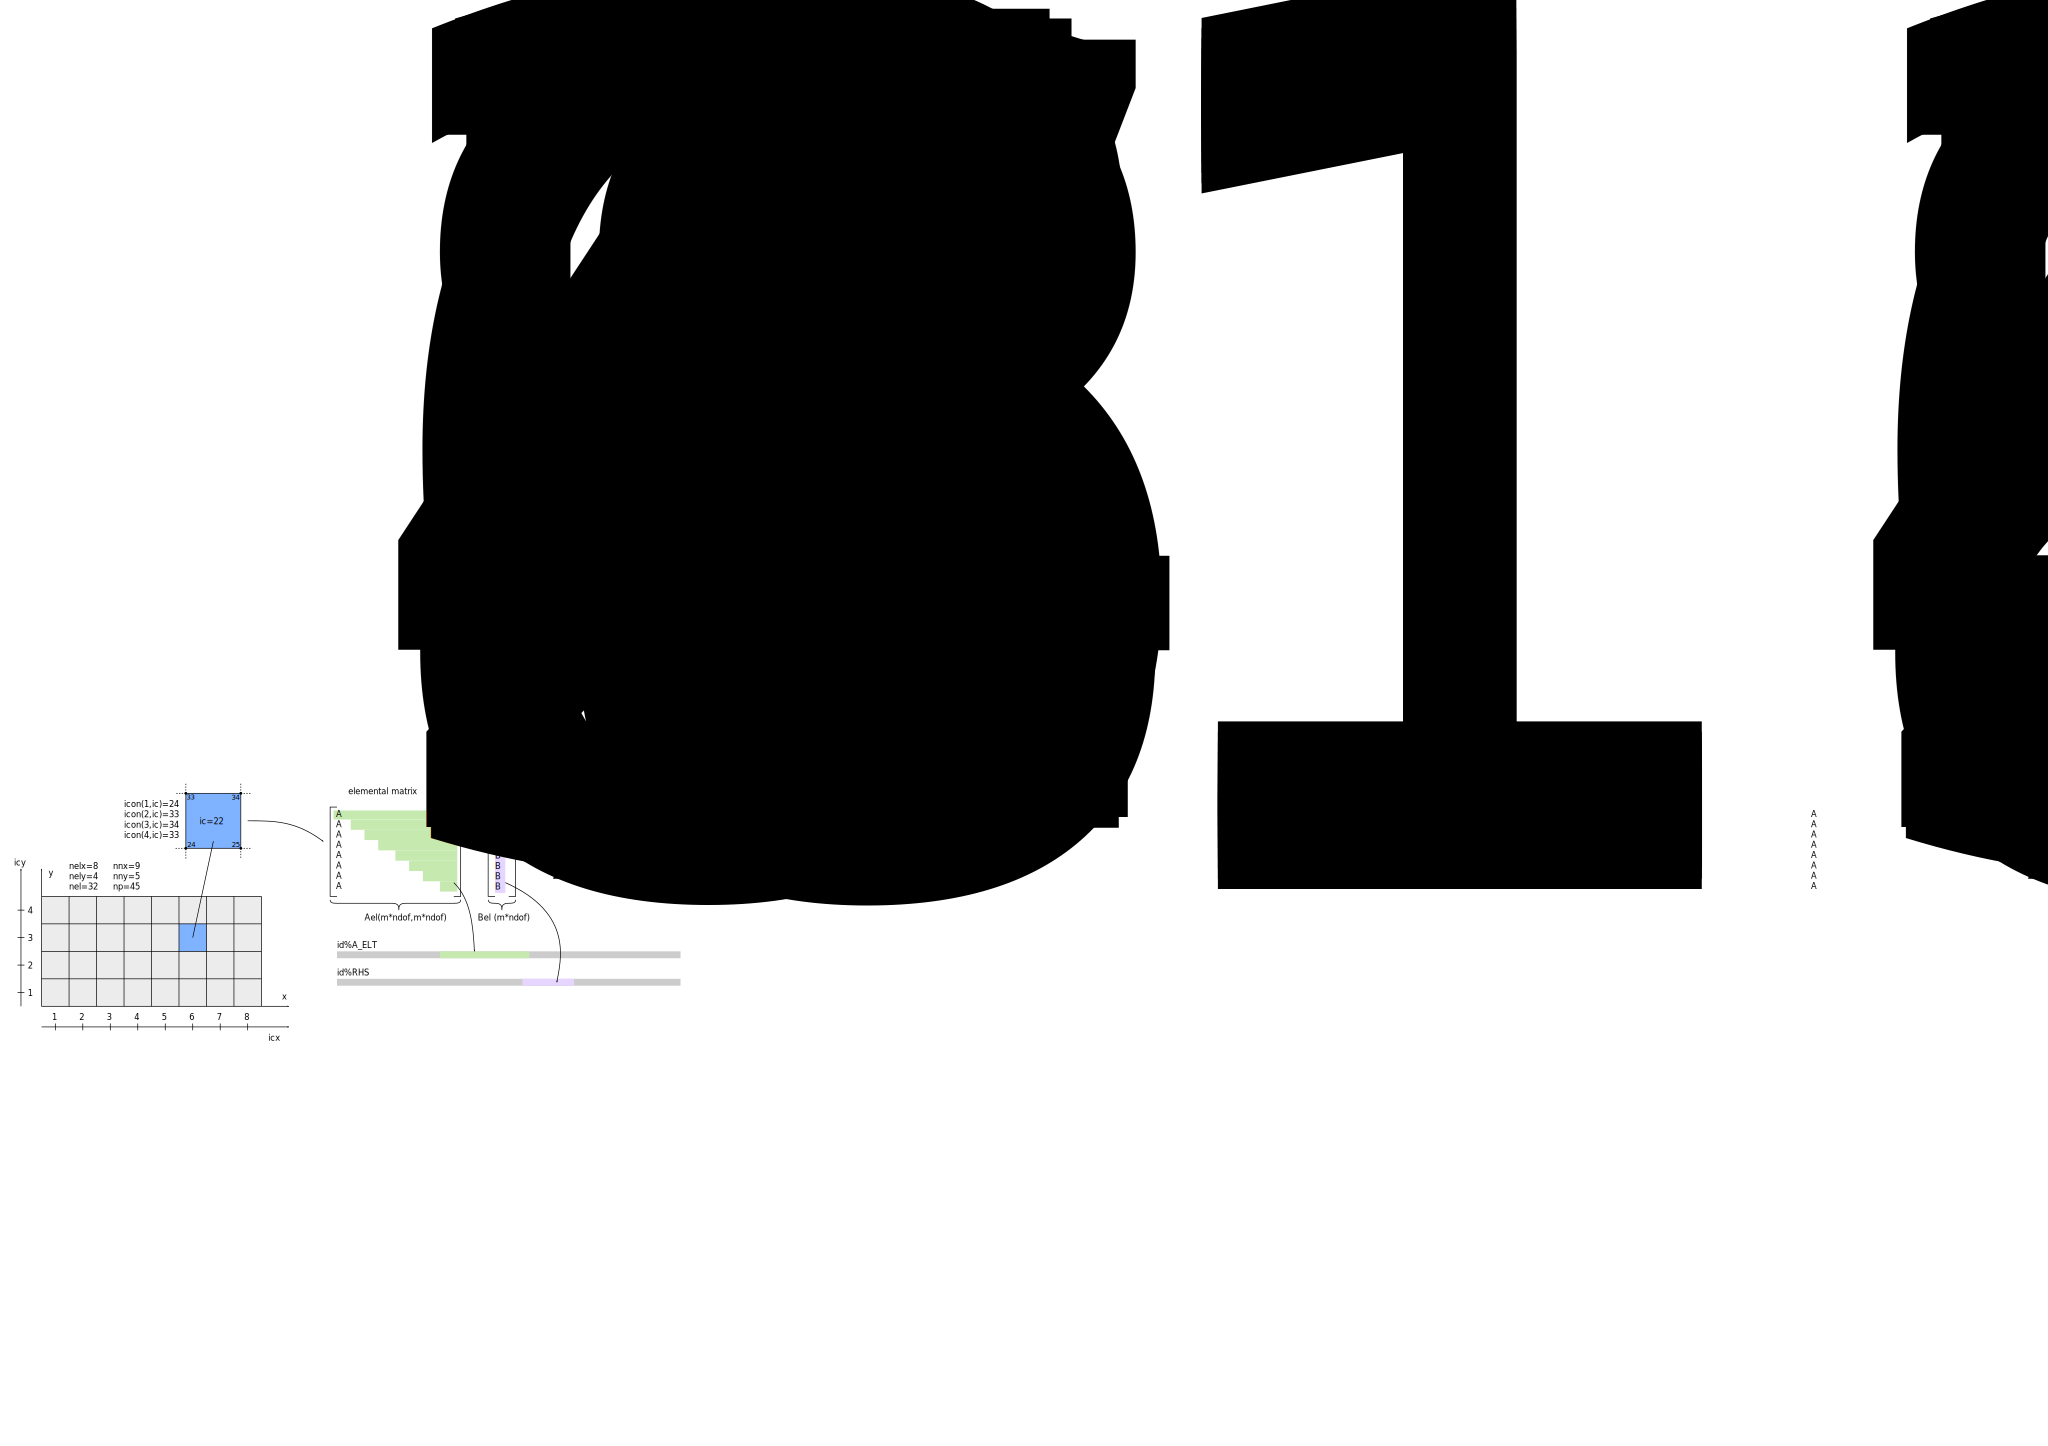
\includegraphics[width=5.cm]{images/sinking_block/FS/stone93/grid}
\includegraphics[width=5.cm]{images/sinking_block/FS/stone93/u}
\includegraphics[width=5.cm]{images/sinking_block/FS/stone93/vel}\\
\includegraphics[width=5.cm]{images/sinking_block/FS/stone93/v}
\includegraphics[width=5.cm]{images/sinking_block/FS/stone93/press}
\includegraphics[width=5.cm]{images/sinking_block/FS/stone93/sr}
\end{center}

\begin{center}
\includegraphics[width=5.6cm]{images/sinking_block/u_FS}
\includegraphics[width=5.6cm]{images/sinking_block/v_FS}
\includegraphics[width=5.6cm]{images/sinking_block/pressure_FS}
\end{center}

\paragraph{No-slip boundary conditions}.

\begin{center}
\includegraphics[width=5.6cm]{images/sinking_block/u_NS}
\includegraphics[width=5.6cm]{images/sinking_block/v_NS}
\includegraphics[width=5.6cm]{images/sinking_block/pressure_NS}
\end{center}








